\section{Лабораторная работа 1 \\ Определение теплоты гидратации сульфата меди}
\textbf{Тема:}
\textbf{Цель работы:}
Определить   теплоту   растворения  безводной соли и её кристаллогидрата. Вычислить теплоту растворения  по закону Гесса.

\textbf{Оборудование и реактивы:} калориметр, магнитная мешалка, секундомер, 5г $KCl$, 2,5 г $CuSO_{4}$(безводный) 2,5 $CuSO_{4}\cdot 5H_{2}O$, стакан на     250 мл.

Все работы  проводят  с  использованием  прибора,   являющегося основным прибором в термохимии и называемого калориметром. Он позволяет определять тепловые эффекты различных физико-химических величин.

Простейший калориметр изображен на рисунке. Химический стакан 3, в котором проводится растворение золи, помещают в толстостенный (батарейный) стакан 1.  Это необходимо  для того, чтобы теплота, выделяющаяся при поглощении, в процессе растворения не терялась в окружающую среду,  а так же не поступала из нее.

Стакан 1 покрывают крышкой с двумя  отверстиями:  одно для термометра 2,  другое для пробирки 5 с навеской растворяемой соли. Для удобства работы пробирка не имеет дна.  Ее нижний конец закрывает  резиновой  пробкой 6 с монтированной в нее металлической палочкой.  В нужный момент это обеспечивает быстрое  высыпание  соли для ее растворения.
Калориметр устанавливают на магнитную мешалку 4.  
\begin{figure}[h]
\center{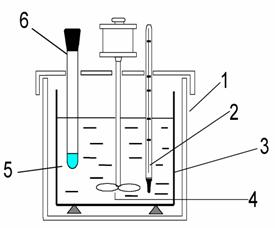
\includegraphics[width=0.25\linewidth]{ris1.jpg}}
\caption{Калориметр с магнитной мешалкой}
\label{ris:image}
\end{figure}

\textbf{Порядок выполнения}

1. Собрать прибор в соответствии с рисунком.

2. Определить постоянную калориметра $K$.

Постоянная калориметра $K$ выражает то количество тепла,  которое необходимо подвести к участвующей в  тепловом  обмене  части калориметра, чтобы повысить его температуру на 1 градус. Для определения постоянной калориметра пользуются кристаллическим хлоридом калия ($KCl$). Необходимо взвесить  на технических весах 2,5 г хлорида калия,  предварительно растертого в ступке, и перенести его в пробирку (3) с пробкой.

Налить в стакан (4) 125 мл воды,  температура которой примерно на 3 $^{o}$C ниже комнатной.
 
Включить мешалку и в течении 20 минут записывать показания термометра с точностью 0.05 град через каждую минуту. На 10-ой минуте, не изменяя температуру,  выталкивают палочкой пробку из пробирки 3 с солью так,  чтобы вся соль высыпалась в воду, и. начиная с 11-ой минуты, вновь каждую минуту делают 10 замеров температуры. Результаты измерений заносят в столбец 3 таблицы (20 строк). 

3. Определить теплоту растворения безводного сульфата меди $Q_{1}$.

Выполнить аналогично п.2 с навеской 2,5 г безводного сульфата меди  ($CuSO_{4}$(безводный)). Результаты измерений заносят в столбец 4 таблицы (20 строк).

4. Определяем теплоту растворения кристаллогидрата $Q_{2}$

Выполнить аналогично п.2 с навеской 2,5 г безводного сульфата меди ($CuSO_{4}\cdot 5H_{2}O$). Результаты измерений заносят в столбец 5 таблицы (20 строк).

\begin{table}[h]
\caption{Экспериментальные данные}
\label{tabular:data1}
\begin{center}
\begin{tabular}{|c|p{4cm}|p{4cm}|p{4cm}|p{4cm}|}
\hline
\No & Время от начала опыта, мин & Навеска $KCl$, $^{o}$C & Навеска $CuSO_{4}(\textrm{безвод.})$, $^{o}$C & Навеска $CuSO_{4}\cdot 5H_{2}O (\textrm{безвод.})$, $^{o}$C\\
\hline
1 & 2 & 3 & 4 & 5 \\
\hline
1 & & & & \\
\hline
 & & & & \\
\hline
20 & & & & \\
\hline
\end{tabular}
\end{center}
\end{table}
\textbf{Обработка экспериментальных данных}

В ходе опыта происходит теплообмен с  окружающей  средой,  т.к. температура воды отличается от комнатной температуры и имеет место выравнивание температур. Поэтому, определить  точную величину изменения температуры ($\Delta t$) при растворении соли по данным, полученным в результате опыта, можно только графическим методом.  График строят в координатах температура --- время.  После нанесения на график всех экспериментально полученных точек, большее число их соединяют прямыми, которые продолжают их до пересечения с перпендикуляром,  восстановленным в 10-ю минуту.  Отрезок, отсекаемый на перпендикуляре, соответствует изменению температуры ($\Delta t$).

Постоянную калориметра вычислить по уравнению:
$$K=\frac{mQ}{M\Delta t}$$

где $m=2,5$г - масса $KCl$; $M$ - молярная масса $KCl$, (г/моль); $Q=18,826$ кДж/моль - молярная  теплота растворения для  $KCl$;

Молярную теплоту растворения безводного сульфата меди ($Q_{1}$) и молярную теплоту растворения кристаллогидрата ($Q_{2}$) вычислить по уравнению:
$$Q_{1}=\frac{K\Delta t_{1}M_{1}}{m_{1}}$$
$$Q_{2}=\frac{K\Delta t_{2}M_{2}}{m_{2}}$$
где $m_{1}=m_{2}=2,5$г - масса навесок соли; $M_{1}$, $M_{2}$ - молярная масса соли, (г/моль);

Вычислить теплоту гидратации ($Q_{3}$) при помощи закона Гесса.
$$CuSO_{4}+5H_{2}O=CuSO_{4}\cdot 5H_{2}O+Q_{3} $$
$$CuSO_{4}=CuSO_{4}(aq)+Q_{1} $$
$$CuSO_{4}\cdot 5H_{2}O= CuSO_{4}(aq)+5H_{2}O+Q_{2}$$
\textbf{Контрольные вопросы}
\begin{enumerate}
\item Что такое тепловой эффект химической реакции?
\item Дайте формулировку закона Гесса.
\item Что  называется  теплотой  (энтропией) образования,  теплотой сгорания? При каких условиях они считаются стандартными?
\item Как по теплоте образования и теплоте сгорания вычислить тепловой эффект реакции?
\item Что понимается под теплотой растворения, теплотой гидратации?
\item Из каких тепловых эффектов складывается  теплота  растворения твёрдого вещества?
\item Что учитывает постоянная калориметра и как её определить?
\item Как определить изменение температуры при растворении?
\end{enumerate}
